\documentclass[fontsize=14pt,DIV=1,numbers=withenddot,twoside=off]{scrartcl}
\usepackage{fontspec,xltxtra,xunicode} 

\setsansfont[Scale=MatchLowercase, Ligatures=TeX]{Arial} 
\renewcommand{\familydefault}{\sfdefault}

\usepackage{polyglossia}
\setdefaultlanguage[spelling=new]{german}
\usepackage[german=quotes]{csquotes}
\MakeOuterQuote{"}

\usepackage{graphicx}
\usepackage{enumitem}
\usepackage[style=authoryear,backend=biber,autolang=hyphen]{biblatex}
\usepackage[%headsep=.5cm,includehead,
    includefoot,a4paper,lmargin=25mm,rmargin=25mm,tmargin=25mm,bmargin=20mm]{geometry}
\usepackage[%urlcolor=blue,colorlinks=true
]{hyperref}
\urlstyle{sf}
\setlist{noitemsep}

% new command for grouping info about the report
\makeatletter
\def\@reportinfo{}
\newcommand{\reportinfo}[3]{%
  \def\@reportinfo{%
   {\normalsize
    \begin{description}[labelindent=5cm]
     \item[Version] #1
     \item[Cluster] #2
     \item[Verantwortlicher Partner] #3
    \end{description}
  }}
}
\makeatother

% typesetting the title
\makeatletter
    \def\maketitle{%
    \begin{center}
    \setlength{\baselineskip}{30pt}
    {\Huge{\textbf{\@title}}}%
    \end{center}
    \medskip
    \@reportinfo
    }
\makeatother

\newcommand{\deliverable}[3]{%
    \begin{description}
    \item[Verantwortlicher Partner:] #1
    \item[Projektmonat der Ablieferung:] #2
    \end{description}%
    #3}

\title{Platz für den Titel}
\author{N.N.}
\date{\today}
\reportinfo{\today}{Clusternumber}{Your institution}

\bibliography{your_bib_file}
\begin{document}
\pagestyle{empty}
\newgeometry{%headsep=.5cm,footskip=.7cm,
lmargin=20mm,rmargin=20mm,tmargin=25mm,bottom=15mm}

\includegraphics[width=0.55\textwidth]{img/dariah-logo.png}
\vspace{20mm}
\maketitle
\vspace{5mm}
\begin{center}
\begin{LARGE}
\noindent\textbf{DARIAH-DE\\\vspace{3mm}Überführung~der~digitalen Forschungsinfrastrukturen~für~die e-Humanities~in~die Operational~Phase~(Betriebsphase)}
\end{LARGE}
\bigskip\bigskip
\vspace{10mm}

\begin{small}
\noindent Dieses Forschungs- und Entwicklungsprojekt wird / wurde mit Mitteln des Bundesministeriums für Bildung~und~Forschung~(BMBF), Förderkennzeichen 01UG1610A bis J, gefördert und vom Projektträger im Deutschen Zentrum für Luft- und Raumfahrt~(PT-DLR) betreut.\\
\end{small}
\vspace{20mm}

\includegraphics{img/bmbf.png}
\end{center}
\restoregeometry
\newpage
\normalsize
\begin{description}
\item[Projekt:] DARIAH-DE: Überführung der digitalen Forschungsinfrastrukturen für die e-Humanities in die Operational Phase (Betriebsphase)
\item[BMBF Förderkennzeichen:] 01UG1610A bis J
\item[Laufzeit:] März 2016 bis Februar 2019
\end{description}

\begin{description}
    \item[Dokumentstatus] Entwurf% or final
    \item[Verfügbarkeit] DARIAH-DE-intern
    \item[Autoren]
    \begin{itemize}
        \item[ ] % has to remain empty for formatting reasons
        \item[ ] N.\,N.
        \item[ ] N.\,N.
    \end{itemize}
\end{description}

\vspace{15mm}
\noindent\textbf{Revisionsverlauf:}\\
\begin{center}
    \begin{tabular}{l l l}
        Datum & Autor & Kommentare  \\
        30.11.2016 & N.N. & Vorlage 
    \end{tabular}
\end{center}



\vfill
\noindent\includegraphics[width=0.13\textwidth]{img/by.eps}

\noindent Dieses Werk ist unter einer Creative Commons Lizenz vom Typ Namensnennung 3.0 Deutschland zugänglich. Um eine Kopie dieser Lizenz einzusehen, konsultieren Sie http://creativecommons.org/licenses/by/3.0/de/ oder wenden Sie sich brieflich an Creative Commons, Postfach 1866, Mountain View, California, 94042, USA.

\newpage
\pagestyle{plain}
\tableofcontents
\section{Einleitung}

\section{Mitte}

\section{Schluß}

\end{document}

%%% Local Variables:
%%% mode: latex
%%% TeX-master: t
%%% TeX-PDF-mode: t
%%% TeX-engine: xelatex
%%% End:
